\documentclass[12pt]{beamer}
\usetheme[navbar=false, bkgimage=false, shadow=true]{Fermi}

\usepackage{graphicx}

\usepackage{amsmath}
\usepackage{xspace}
\usepackage{deluxetable}

\newcommand{\gtlike}{\ensuremath{\mathtt{gtlike}}\xspace}
\newcommand{\pointlike}{\ensuremath{\mathtt{pointlike}}\xspace}
\newcommand{\gtobssim}{\ensuremath{\mathtt{gtobssim}}\xspace}
\newcommand{\fermi}{\textit{Fermi}\xspace}

\title{Search for Spatially Extended \fermi-LAT Sources Using Two Years of Flight
Data}
%\subtitle{\ldots}

\author{Joshua Lande}
\institute{SLAC/Stanford}
\email{joshualande@gmail.com}
\date{August 25, 2011}

\begin{document}

\fermititle

\begin{frame}{Overview}
  \begin{itemize}
    \item Category II Paper
    \item Contact Authors: J. Lande, M. Ackermann, S. Funk
    \item Internal Referees: Marianne Lemoine-Goumard and Johann Cohen-Tanugi
    \item Target Journal: ApJ
    \item Currently submitted to internal referees
    \item Feedback welcome
  \end{itemize}
\end{frame}

\begin{frame}{Paper Outline}
  \begin{itemize}
    \item Description of a new method (\texttt{pointlike}) for analyzing extended sources.
    \item Monte Carlo calculation of false detection rate for extended sources.
    \item Calculation of the LAT's detection threshold 
      to spatially extended sources
    \item Presentation of a new search for spatially extended sources:
      \begin{itemize}
        \item Reanalyzing extension of 12 extended sources in 2FGL
        \item Test AGN from 2LAC for extension to validate the analysis
        \item Present 9 extended sources not in 2FGL
      \end{itemize}
  \end{itemize}
\end{frame}



\begin{frame}{Fig. 1}
  \begin{center}
    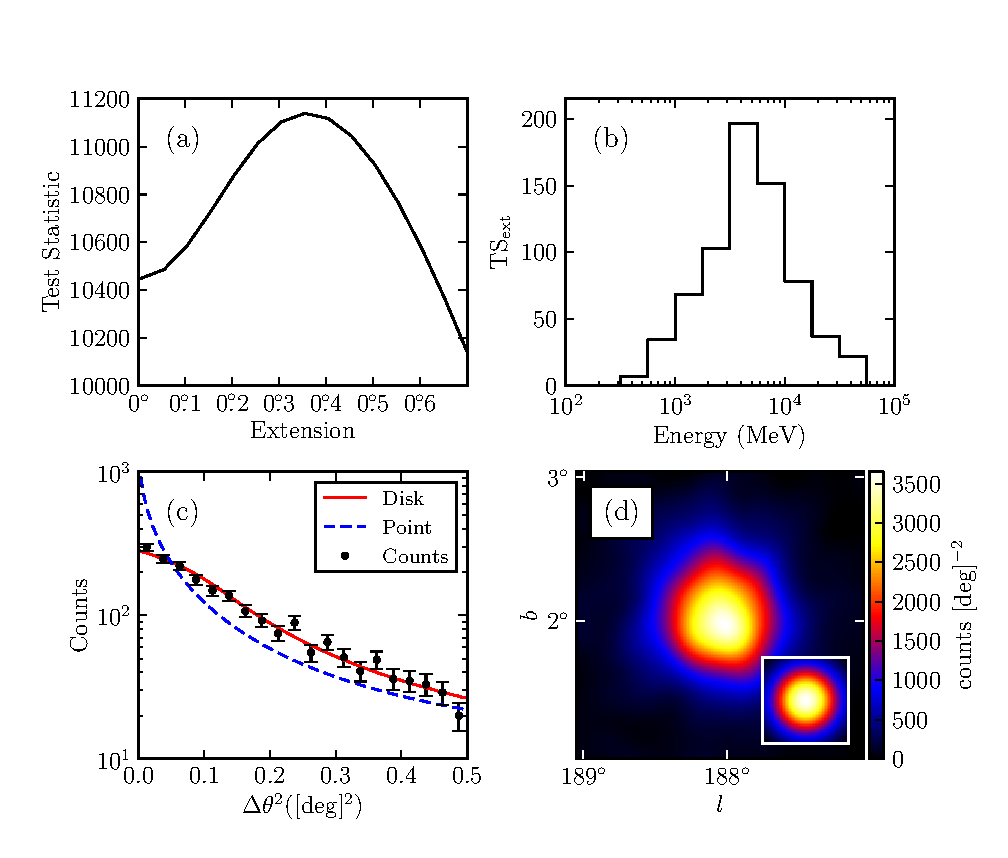
\includegraphics[scale=0.5]{../paper/ic443_plots/four_plots_ic443_color.eps}
  \end{center}
\end{frame}

\begin{frame}{Fig. 2}
  \begin{center}
    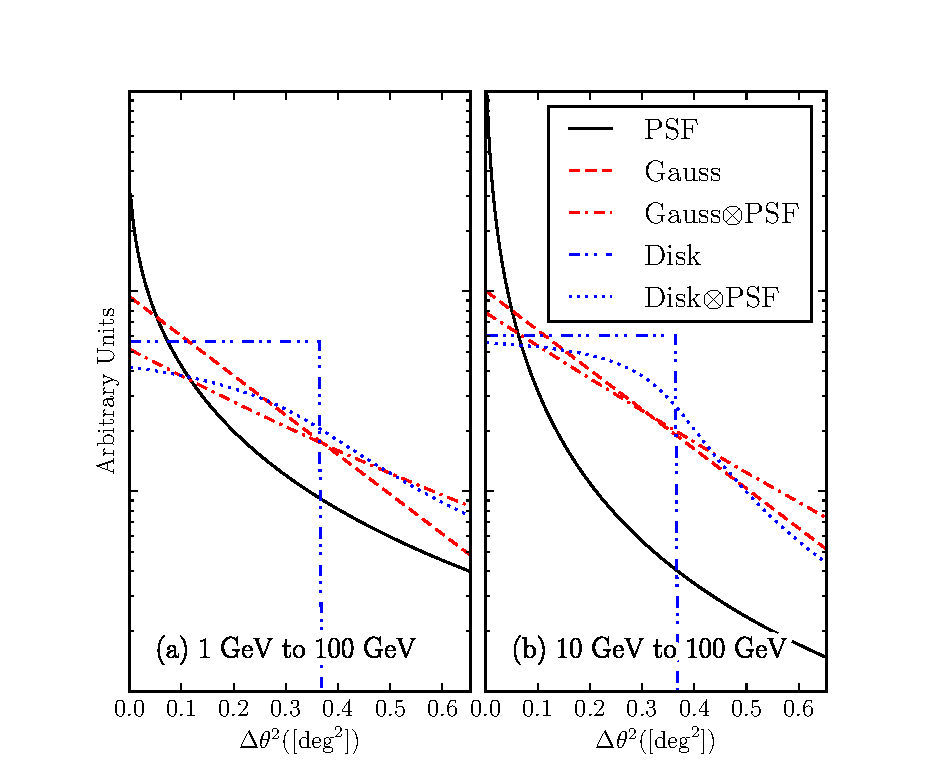
\includegraphics[scale=0.5]{../paper/mc_plots/compare_disk_gauss_color.eps}
  \end{center}
\end{frame}

\begin{frame}{Fig. 3}
  \begin{center}
    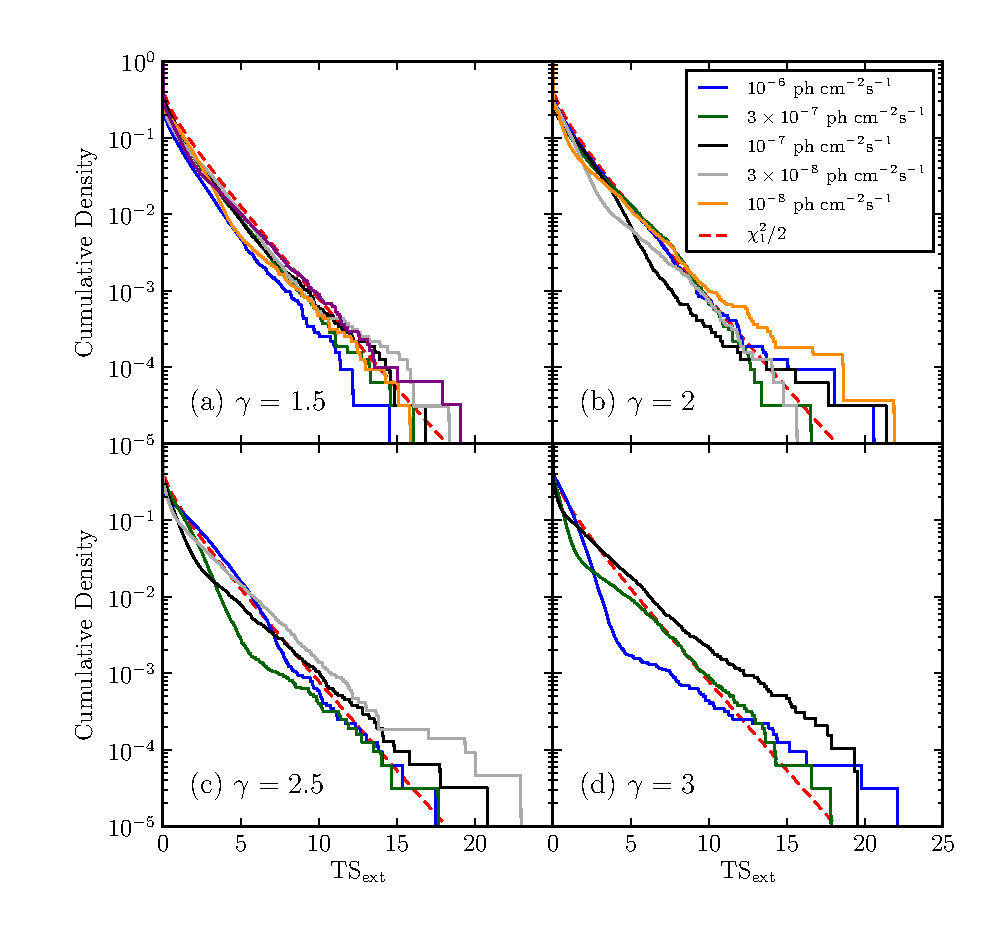
\includegraphics[scale=0.5]{../paper/mc_plots/ts_ext_emin_1000_color.eps}
  \end{center}
\end{frame}

\begin{frame}{Fig. 4}
  \begin{center}
    \includegraphics[scale=0.5]{../paper/mc_plots/index_sensitivity_color.eps}
  \end{center}
\end{frame}

\begin{frame}{Fig. 5}
  \begin{center}
    \includegraphics[scale=0.5]{../paper/mc_plots/all_sensitivity_color.eps}
  \end{center}
\end{frame}

\begin{frame}{Fig. 6}
  \begin{center}
    \includegraphics[scale=0.5]{../paper/mc_plots/time_sensitivity_color.eps}
  \end{center}
\end{frame}

\begin{frame}{Fig. 6}
  \begin{center}
    \includegraphics[scale=0.5]{../paper/mc_plots/time_sensitivity_color.eps}
  \end{center}
\end{frame}


\begin{frame}
  \begin{center}
    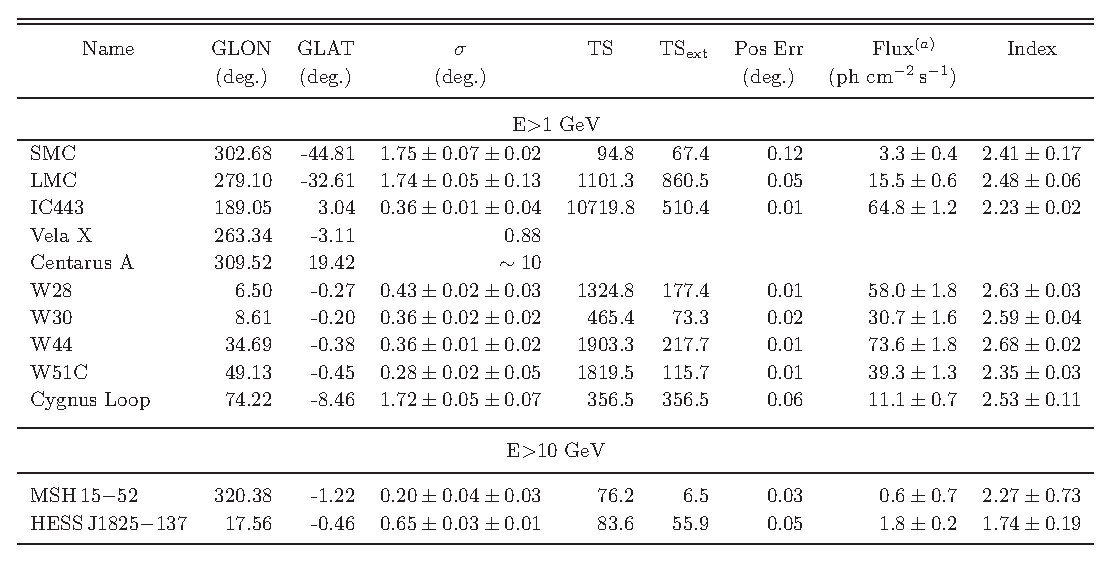
\includegraphics[scale=0.5]{tables/table3.eps}
  \end{center}
\end{frame}

\begin{frame}
  \begin{center}
    \includegraphics[scale=0.5]{tables/table4.eps}
  \end{center}
\end{frame}

\begin{frame}
  \begin{center}
    \includegraphics[scale=0.5]{tables/table5.eps}
  \end{center}
\end{frame}

\end{document}
